\section{Experiments and Results}
\label{sec:experiments}

In our experiments, we evaluate the VITA-E framework's capabilities across a set of interactive scenarios. We specifically aim to demonstrate its proficiency in: 1) executing fundamental manipulation tasks, 2) providing timely spoken responses, 3) performing actions and speech concurrently, 4) handling dynamic task switching, and 5) responding to emergency stop commands. 

Our experiments are conducted on a Fourier GR2 humanoid robot platform~\citep{FourierGR2}. The system's input consists of visual data from a first-person-view static Realsense D455 RGB camera mounted on the robot's head, along with the robot's proprioceptive states.

\subsection{Fundamental Manipulation Tasks}

\textbf{Simulation experiments.} To establish a baseline for manipulation capability, we first evaluate the model's performance on the Libero benchmark. The Libero benchmark is designed to evaluate a model's ability to apply and transfer action skills, which is composed of four distinct action task suites: Object, Spatial, Goal, and LONG.

We compare our model on the Libero benchmark with the baseline model GR00T~\citep{gr00t}. For a fair comparison, we only replace the VLM of the Eagle-2 model in GR00T with the VITA-1.5, and freeze the VLM part, fine-tuning only the diffusion action expert. We also conduct a LoRA-based fine-tuning experiment, where we finetune the VLM backbone with LoRA and fully fine-tune the diffusion action expert, to verify the impact of freezing the VLM backbone. We first pre-train the model on the Libero-90 dataset, and then finetune it on the mixture of the four action task suites. We report the average success rate of these two models in Figure~\ref{fig:libero_results}.

Experimental results show that our model successfully completes a majority of tasks in the Libero benchmark. However, we acknowledge a performance gap when compared to the GR00T model. While VITA-E excels at object recognition, it exhibits limitations in its understanding of spatial relationships and goal concepts. It is crucial to note that GR00T unfreezes the visual encoder and aligner parameters of its Eagle-2 VLM and jointly optimizes them with the diffusion action model via end-to-end training on a large-scale embodied dataset. In contrast, VITA-E does not leverage such large-scale pre-training and is trained with a totally frozen VLM. Furthermore, VITA-E LoRA experiment shows that finetuning the VLM backbone with LoRA can improve the performance of the model. However, since fine-tuning the VLM backbone can lead to a certain degree of degradation in the model's language abilities, we therefore keep the VLM backbone frozen in our real robot experiments. Overall, the observed disparity in success rates is an expected outcome given these significant architectural and data-related constraints.

\begin{figure}[t!]
    \centering
    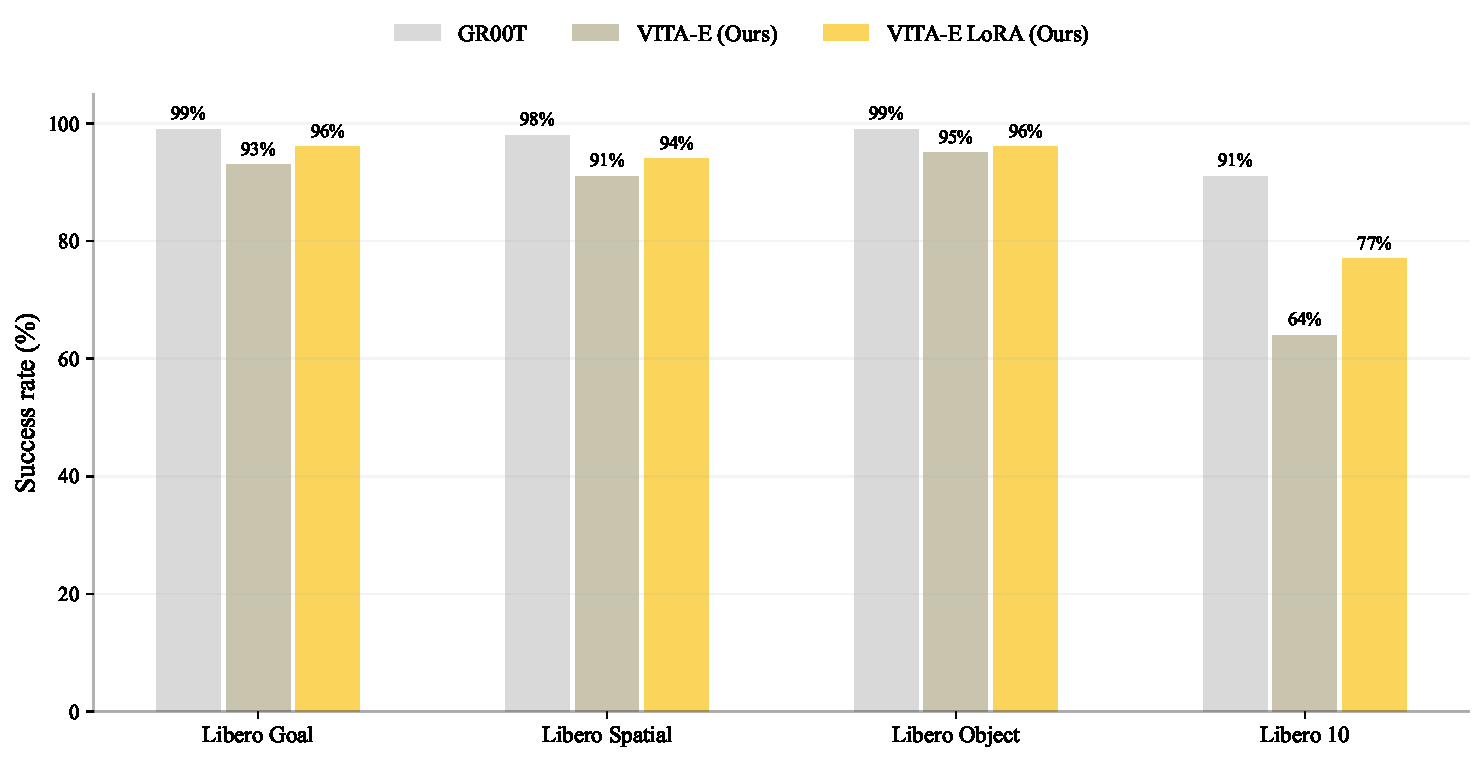
\includegraphics[width=0.8\linewidth]{VITA-E//pic/libero.pdf}
    \caption{Success rate comparison of VITA-E and GR00T on the Libero benchmark. Although the success rates of VITA-E on this benchmark are not as good as the baseline with the same structure, we emphasize that the goal of this work is not for VITA-E to achieve the state-of-the-art experimental performance, but to prove that the model is capable of completing embodied tasks and to provide quantitative metrics.}
    \label{fig:libero_results}
    \vspace{-1.3em}
\end{figure}

\textbf{Real robot experiments.} To demonstrate the model's capabilities on the real robot, we evaluate the model's fundamental pick-and-place skills across two scenarios: 1) picking up a can from the table, and 2) picking up a toy and placing it into a basket. For each task, we collect 300 demonstrations by teleoperating the robot arm at 20 Hz across 26 degrees of freedom.

To show the performance of our method, we select several state-of-the-art models and train them on our collected dataset. For $\pi_0$~\citep{pi0} and Diffusion Policy~\citep{dp}, we train the entire model. For GR00T~\citep{gr00t} and SmolVLA~\citep{smolvla}, we train their entire action expert modules. In contrast, and to mitigate overfitting, we fine-tune only the action projector of VITA-E. We evaluate each method for 30 trials to obtain the final success rate, as reported in Figure~\ref{fig:basic_results}.

\begin{figure}[t!]
    \centering
    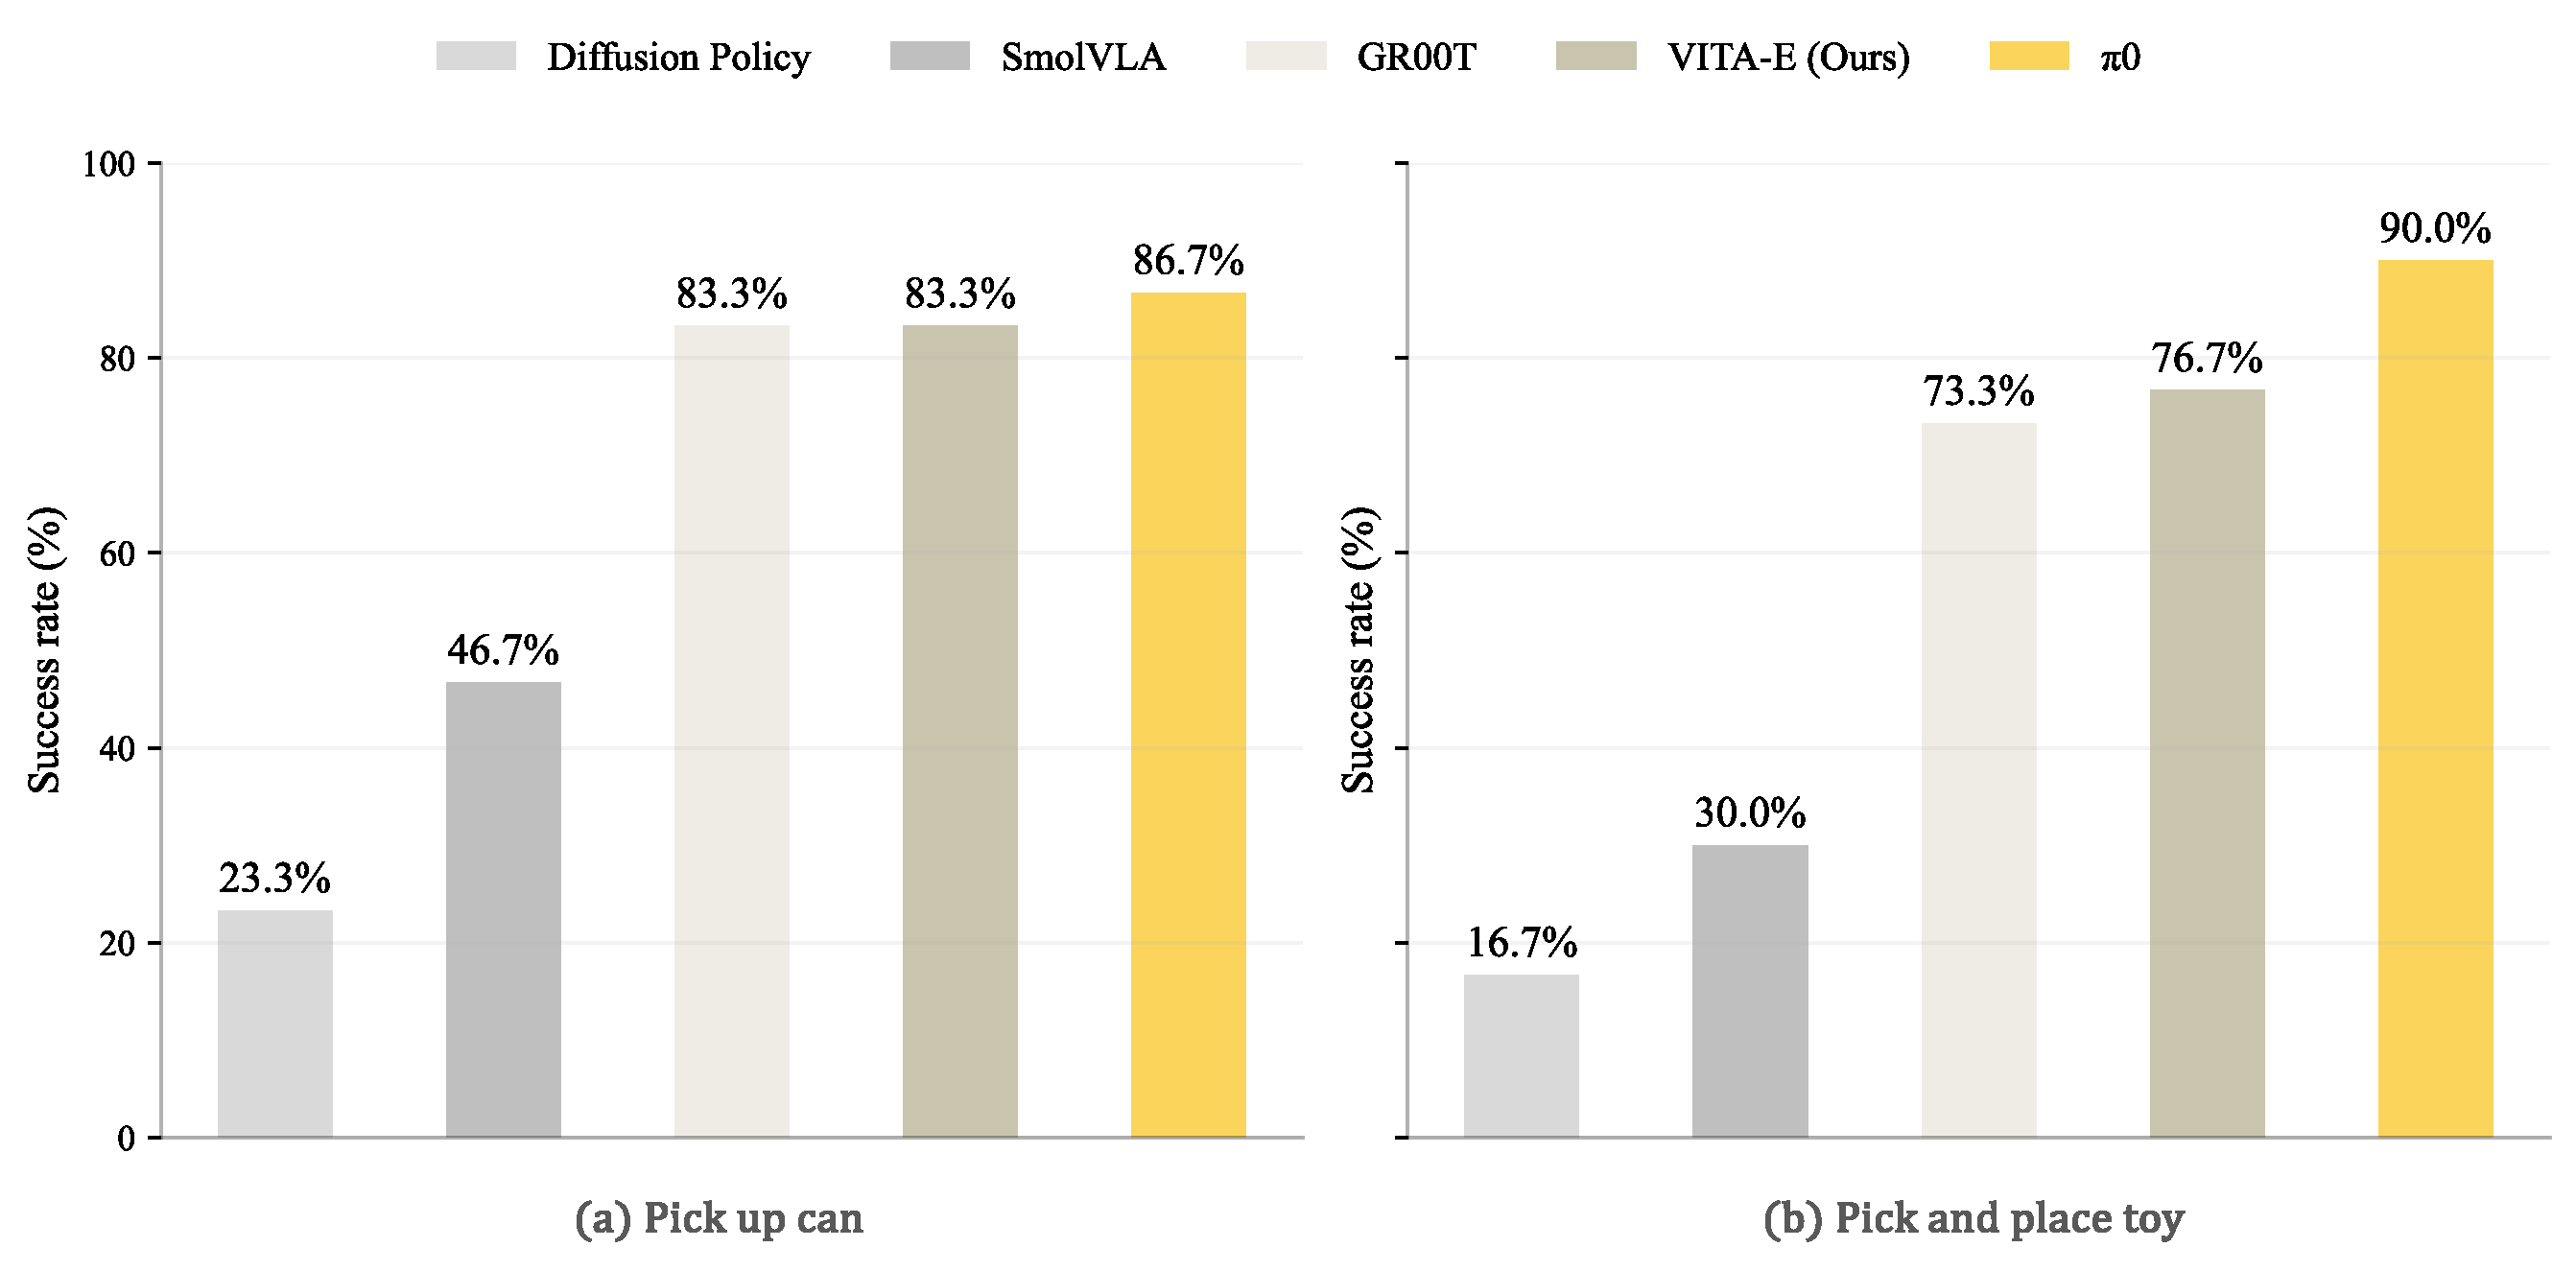
\includegraphics[width=0.8\linewidth]{VITA-E//pic/results.pdf}
    \caption{Success rate comparison of VITA-E and baseline models on two fundamental manipulation tasks: (a) Pick up can and (b) Pick and place toy. Results are reported over 30 evaluation trials.}
    \label{fig:basic_results}
    \vspace{-2em}
\end{figure}

The results demonstrate that VITA-E is a highly capable manipulation model, whose performance is on par with state-of-the-art models. While the goal is not to outperform the top manipulation-focused baselines, these results confirm that our system's core capabilities are sufficiently strong to reliably evaluate our primary contribution: a novel architecture for real-time human-robot interaction. Moreover, it is equally worth emphasizing that our architecture remains compatible with dual-system VLA models such as $\pi_0$.

\subsection{Interactive Tasks}

The core contribution of our work lies in enabling natural human-robot interaction. We evaluate VITA-E on four critical interactive capabilities: speech-action concurrency, speech interruption, action switching, and emergency stops. We evaluate the concurrency skill qualitatively, while we measure the other three by their success rate in 30 trials. As the baseline methods evaluated in the previous section are not designed with analogous real-time interaction capabilities, our evaluation of these tasks focuses exclusively on our proposed framework.

For the concurrency task, we observe that VITA-E can consistently provide spoken answers to user queries while smoothly continuing its manipulation task, without any noticeable pauses or degradation in its physical execution. The average latency of VITA-E's voice responses across ten tests is 2.26s. The quantitative results for the other tasks are reported in Table~\ref{tab:interactive-tasks}. The results show that VITA-E achieves a perfect 100\% success rate in both interrupting its own speech and in the emergency stop task. This near-perfect performance validates the effectiveness of our dual-model architecture in achieving instantaneous system-level interruption capabilities.

\begin{table}[h]
    \vspace{-2em}
    \caption{Success rates on interactive tasks (30 trials).}
    \label{tab:interactive-tasks}
    \centering
    \resizebox{0.7\linewidth}{!}{%
    \begin{tabular}{@{}lccc@{}}
        \toprule
        \textbf{Interactive Task} & Speech Interruption & Task Switching & Emergency Stop \\
        \midrule
        \textbf{Success Rate (SR)} & 100\% & 93.3\% & 100\% \\
        \bottomrule
    \end{tabular}%
    }
    \vspace{-2em}
\end{table}

In the more complex task switching scenario, VITA-E achieves a 93.3\% success rate. The few failures are not due to the interruption mechanism itself, but stem from occasional misinterpretations by the VLM. In these cases, the VLM fails to recognize the new user directive as an action command, consequently providing only a verbal response instead of switching its physical task. We believe this problem can be addressed by further expanding the VLM's training with more diverse embodied scenarios. These results nonetheless strongly demonstrate the overall superiority of our framework in handling dynamic, real-time user interventions.

\subsection{Interactive Latency Comparison}

To rigorously evaluate the necessity of our dual-model architecture, we compare VITA-E against two representative single-model baseline strategies: \textbf{Single-VLM Queue}, which processes requests sequentially, and \textbf{Single-VLM Preemption}, which switches tasks immediately upon receiving a new instruction. As summarized in Table \ref{tab:scenario_comparison}, these paradigms are evaluated across three critical dynamic human-robot interaction scenarios.

\textbf{Speech Interruption.} In conversational scenarios, the Single-VLM Queue strategy exhibits extremely high latency. While both Single-VLM Preemption and VITA-E achieve rapid responses, VITA-E accomplishes this seamlessly through its Standby Model, which generates a preemption event to instantly terminate the Active Model's speech generation.

\textbf{Action Switching and Emergency Stop.} The fundamental limitations of single-model paradigms become most apparent during physical manipulation. The Single-VLM Queue is inherently unable to adapt to new action requests once an action sequence has begun. Conversely, while the Single-VLM Preemption strategy allows for rapid switching, it is indiscriminately interrupted by any user speech, leading to severe physical instability and safety risks. VITA-E resolves this critical dilemma by offloading the intent recognition to the Standby Model. The system only interrupts the Active Model's physical execution when the Standby Model explicitly recognizes a command to be executed, such as an emergency stop or a valid new task.

\textbf{Concurrency.} The Single-VLM Queue strategy fails to support concurrency entirely. Furthermore, attempting concurrency via a Single-VLM Preemption strategy results in intermittent actions due to constant computational resource contention between speech and action generation. VITA-E effectively breaks this bottleneck. When the Active Model is executing a physical task, it enters a protected state. A new conversational query is handled by the Standby Model, which generates a voice response without interrupting the ongoing physical task. This parallel processing allows the robot to consistently provide verbal responses without any noticeable pauses or degradation in its physical execution.

\begin{table}[htbp]
    \vspace{-1.5em}
    \centering
    \caption{Performance Comparison in Interruption and Concurrency Scenarios}
    \resizebox{\textwidth}{!}{%
    \setlength{\tabcolsep}{8pt}
    \begin{tabular}{l@{\hspace{1.2em}}c@{\hspace{1.2em}}c@{\hspace{1.2em}}c}
        \toprule
        \textbf{Scenario} & \textbf{Single-VLM Queue} & \textbf{Single-VLM Preemption} & \textbf{VITA-E (Ours)} \\
        \midrule
        \textbf{Speech Interruption} & \textcolor{red}{Extremely high latency} & \textcolor{green!50!black}{Rapid response} & \textcolor{green!50!black}{Rapid response} \\
        \midrule
        \textbf{Action Switching/Stopping} & \textcolor{red}{Extremely high latency} & \textcolor{red}{\makecell[c]{Rapid switch, but \\ interrupted by any requests}} & \textcolor{green!50!black}{\makecell[c]{Rapid switch, only \\ respond to action requests}} \\
        \midrule
        \textbf{Concurrency} & \textcolor{red}{Unable} & \textcolor{red}{Intermittent action} & \textcolor{green!50!black}{Smooth action} \\
        \bottomrule
    \end{tabular}
    }
    \label{tab:scenario_comparison}
    \vspace{-2em}
\end{table}

\subsection{Ablation Studies}

To validate the effectiveness of our fine-tuning strategy for teaching the VLM to act as a system controller, we conduct an ablation study. We compare our fine-tuned \textbf{VITA-E VLM} against its base model, \textbf{VITA-1.5}~\citep{vita15}, on its ability to generate correct responses to user instructions like a robot. The models are prompted to act as a robot, and the accuracy of their responses, as judged by human evaluators, is shown in Table~\ref{tab:ablation}.

\begin{table}[h]
    \vspace{-1.5em}
	\caption{Ablation study: Accuracy of the VLM in generating appropriate responses and control tokens before and after fine-tuning.}
	\label{tab:ablation}
	\centering
	\resizebox{0.7\linewidth}{!}{%
	\begin{tabular}{@{}lccccc@{}}
		\toprule
		\textbf{Model} & \begin{tabular}[c]{@{}c@{}}Cannot \\ Execute\end{tabular} & \begin{tabular}[c]{@{}c@{}}Exec. \\ Inst. 1\end{tabular} & \begin{tabular}[c]{@{}c@{}}Exec. \\ Inst. 2\end{tabular} & \begin{tabular}[c]{@{}c@{}}Emergency \\ Stop\end{tabular} & \begin{tabular}[c]{@{}c@{}}Task \\ Completed\end{tabular} \\ \midrule
		VITA-1.5 (Base) & 75\% & 10\% & 5\% & 0\% & 15\% \\
		\textbf{VITA-E VLM (Ours)} & \textbf{90\%} & \textbf{95\%} & \textbf{95\%} & \textbf{100\%} & \textbf{60\%} \\ 
		\bottomrule
	\end{tabular}%
	}
    \vspace{-2em}
\end{table}

The results show a sharp contrast between the base model and our fine-tuned version. The base VITA-1.5 model can correctly identify nonexecutable instructions with 75\% accuracy, but it performs poorly in generating valid action commands and completely lacks the ability to stop the action. Common failure modes include: 1) explicitly refusing to perform actions with responses like ``I cannot interact with the physical world,'' 2) failing to adopt the specified robot persona, and 3) only describing the steps of a plan rather than directly interacting as a robot.

After fine-tuning on our synthetic dataset, the VITA-E VLM's ability to interpret embodied instructions improves dramatically. It learns to refuse impossible commands with higher accuracy (90\%) and, more importantly, to generate correct action instructions for executable tasks, with accuracy increasing from under 10\% to 95\%. Crucially, the model learns the concept of interruption from scratch, with its accuracy of emergency stop increasing from 0\% to 100\%. This study demonstrates that our targeted fine-tuning is essential for bridging the gap between a general-purpose VLM and a specialized ``model-as-controller" that can reliably control the behaviors of our interactive system.
